\documentclass{article}
\usepackage{tikz}
% A rounded node around a paragraph that breaks into lines: the box height
% depends on the line breaker, and pgfmath's rounded corners read it.
\begin{document}
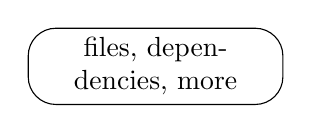
\begin{tikzpicture}
\node[rounded corners=10pt,draw,text width=3cm,align=center] {files, dependencies, more};
\end{tikzpicture}
\gdef\SatexReachedEnd{}
\end{document}
